\section{Modellierung \buch{p.1}}
\subsection{Modellierung eines Embedded Systems \buch{p.3}}

\begin{itemize}
	\item Modelle werden als Werkzeuge der Dokumentation angesehen. Dadruch 
	wird unter Umständen dasselbe zweimal beschrieben (als Code und als Diagramme)
	
	\item Ziel ist es aus formalen Modellen lauffähige Software erzeugt werden kann. Bei 
	State Machine ist dies durch Statechart der Automaten vollständig möglich.
\end{itemize}

\textbf{Agile Softwareentwicklung}\\
Agile Softwareentwicklung ist der Oberbegriff für den Einsatz von Agilität (flink, beweglich) in der Softwareentwicklung.
\begin{itemize}
	\item Eher offen für Änderungen als starres Festhalten an Plänen
	\item Eher Menschen und Kommunikation als Prozesse und Tools
	\item Eher "`darüber miteinander reden"' als "`gegeneinander schreiben"'
	\item Eher Vertrauen als Kontrolliren
	\item Eher "`Best Practices"' aus Erfahrung als verordnete Vorgaben
	\item Eher Angemessenheit als Extremismus
	\item \textbf{Aber keine Anarchie!}
\end{itemize} 


\textbf{Model Driven Development}\\
Bei der modellbasierten Entwicklung kommen in allen Entwicklungsphasen durchgängig Modelle zur Anwendung.

\begin{multicols}{2}
	\textbf{UML:}
	\begin{itemize}
		\item Aktivitätsdiagramm
		\item Sequenzdiagramm
		\item Zustandsdiagramm
		\item Klassendiagramm
		\item Use Case Diagramm
		\item Verteilungsdiagramme
	\end{itemize}
	\columnbreak
	
	\textbf{Vorgehen bei Modellierung:}
	\begin{enumerate}
		\item Systemgrenze Definieren
		\item Systemprozesse finden
		\item Verteilung festlegen
		\item Systemprozesse detaillieren
	\end{enumerate}
\end{multicols}

\subsection{Systemgrenze definieren \buch{p.14}}
Das wichtigste und allererste bei sämtlichen Systemen ist die Festlegung der Systemgrenze (System boundary)
\begin{itemize}
	\item Was macht das System, d.h was liegt innerhalb der Systemgrenze
	\item Mit welchen Teilen ausserhalb des Systems kommuniziert das System
	\item Welches sind die Schnittstellen zu den Nachbarsystemen
\end{itemize}

\begin{figure}[h]
	\centering
	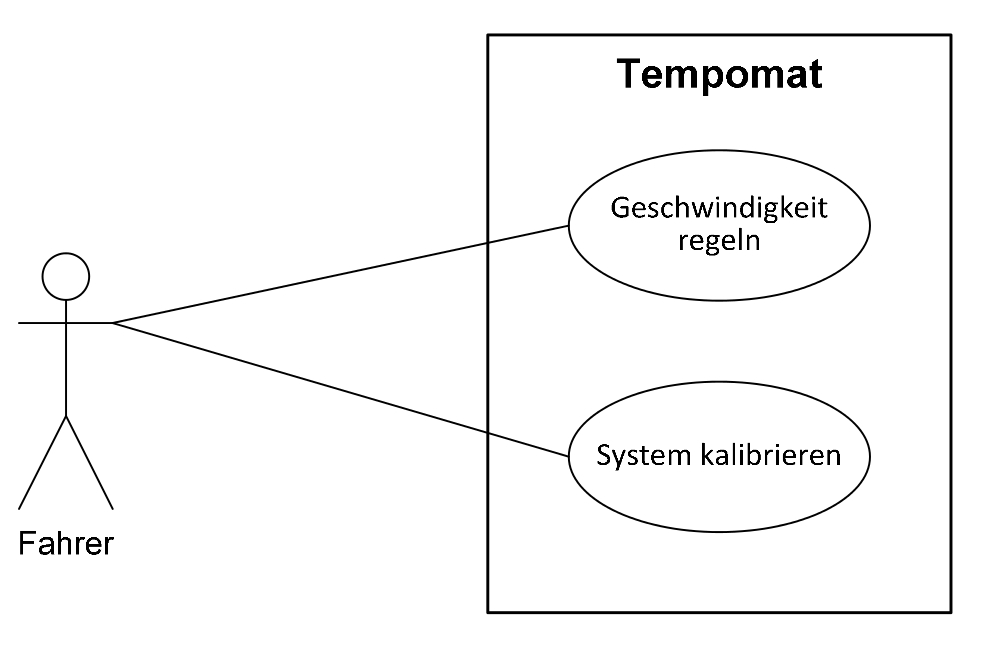
\includegraphics[height=8cm, width = 10cm,]{images/Modellierung/Systemgrenze}
	\caption{Aktoren sind: Menschen, Sensoren, Ein- und Ausgabegeräte, Nachbarsysteme, Zeit.}
\end{figure}


\textbf{Systemprozesse finden}\\
Die Aufteilung in Hardware und Software sollte erst nach der Analyse der grundlegenden Anforderungen erfolgen.
RTE-Systeme bestehen meistens nur aus einem einzigen Systemprozess, speziell wen das System im Prinzip "nur" ein
Regler ist. Dieser Schritt ist in der Analysephase. Wenn hier von Prozessen die Rede ist, bedeutet das nicht unbedingt ein
Betriebssystem Prozess ist.\newline

\subsection{Verteilung Festlegen \buch{p.23}}
Bei Systemen bei denen die Grenze durch Nachrichtenflüsse charakterisiert werden können, eignen sich Sequenzdiagramme
für Kontextbeschreibung.\\

Bei Embedded System werden häufig mehrere Rechner Systeme verwendet um die Aufgaben zu erledigen. Diese liegen meistens 
geographisch (cm bis km) verteilt und sind mit einem Kommunikationskanal verbunden. Diese Systeme heissen Verteilte Systeme 
(Distributed System). Zur Darstellung eignet sich in UML das Verteilungsdiagramm (Deployment Diagramm).\\

\textbf{Verteilungsdiagramm (Distributed System)}
\begin{itemize}
	\item Die Knoten werden zur Darstellung der geographischen Orten oder Subsysteme verwendet
	\item Die physikalische Verbindung zwischen zwei Knoten werden als Linien dargestellt.
	\item Die Knoten können auch hierarchisch aufgebaut sein.
\end{itemize}

\begin{figure}[h]
	\centering
	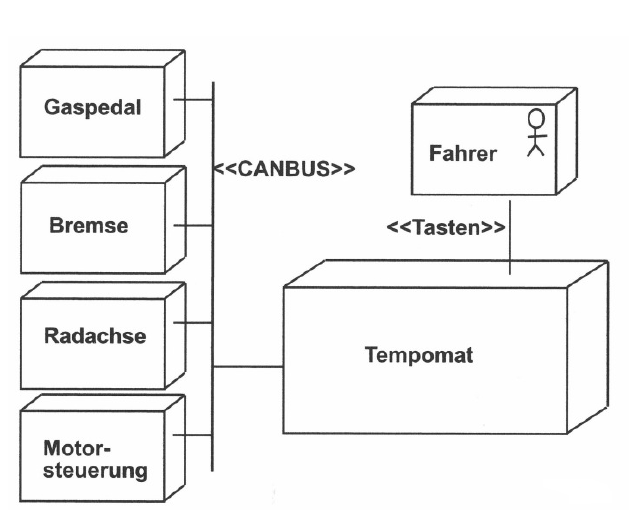
\includegraphics[height=6cm, width = 9cm,]{images/Modellierung/Verteilungsdiagramm}
	\caption{Verteilungsdiagramm}
\end{figure}

\subsection{Systemprozesse Detaillieren \buch{p.27}}
Die Systemprozesse nicht detaillierter spezifizieren als sinnvoll. Je weiter Detaillierung soll einen "`added value"' liefern. 
Leitidee: Lieber weniger als mehr Detail\\

\textbf{Detaillierungsgrad}
\begin{itemize}
	\item \textbf{Überblick: } z.B in Form von normalem umgangssprachlichem Text. Diese Form sollte immer erstellt werden
	\item \textbf{Normale Schicht: } Sie ist für den Systementwickler gedacht und enthält mehr Details  
\end{itemize}

Für die Detaillierung eignen sich Sequenzdiagramm, Aktivitätsdiagramm, Statecharts und Umgangssprachlicher Text.

\subsubsection{Sequenzdiagramme \buch{p.30}}

\begin{multicols}{2}
	\textbf{Zweck:}
	\begin{itemize}
		\item Austausch von Meldungen zwischen Objekten innerhalb einer beschränkten Zeitdauer anzeigen
	\end{itemize}
	\columnbreak
	
	\textbf{Ideal:}
	\begin{itemize}
		\item Für kurze Zeitdauer mit einigen wenigen Objekten
		\item Bei wenigen Verschachtlungen und Verzweigungen
	\end{itemize}
\end{multicols}

\begin{minipage}[hbt]{1cm}
	\centering
	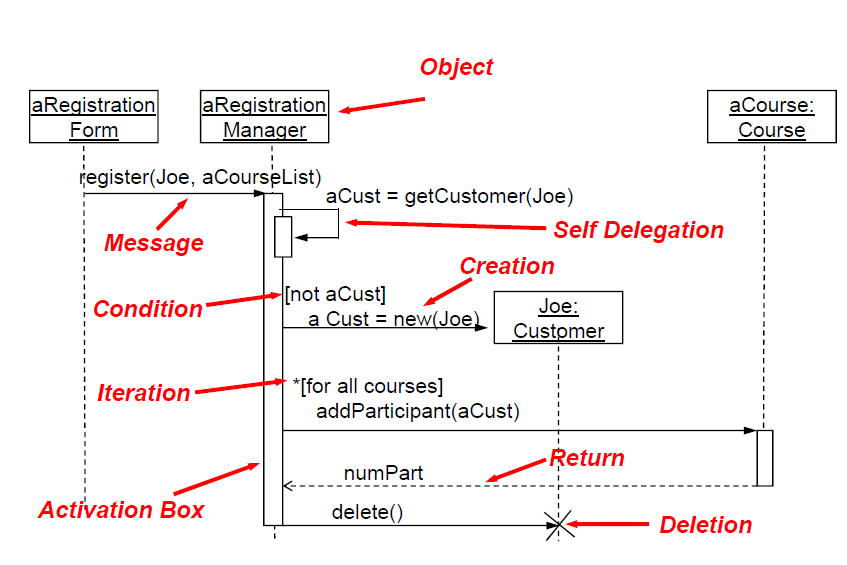
\includegraphics[height=8cm, width = 10cm,]{images/Modellierung/Sequenzdiagramm}
	\label{Bild1}
\end{minipage}
\hfill
\begin{minipage}[hbt]{8cm}
	\centering
	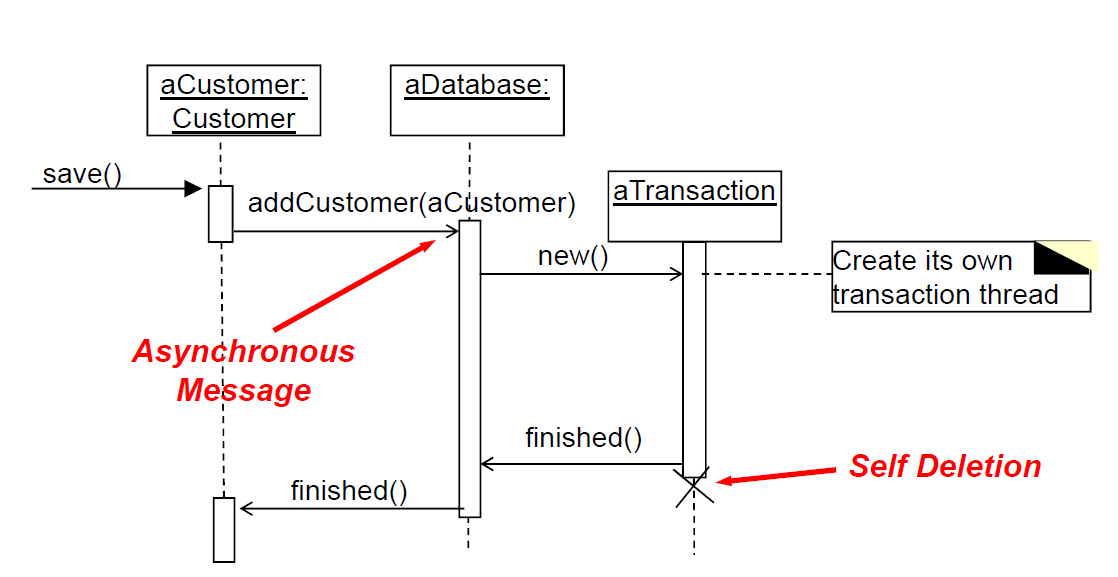
\includegraphics[height=6cm, width = 8cm,]{images/Modellierung/Sequenzdiagramm2}
	\label{Bild2}
\end{minipage}

\newpage
\subsubsection{Kommunikationsdiagramm \buch{41}}
Das Kommunikationsdiagramm zeit dieselbe Information wie das Sequenzdiagramm. Der Schwerpunkt liegt aber
nicht auf dem zeitlichen Ablauf, sondern auf dem Informationsfluss zwischen den Objekten.

\begin{figure}[h]
	\centering
	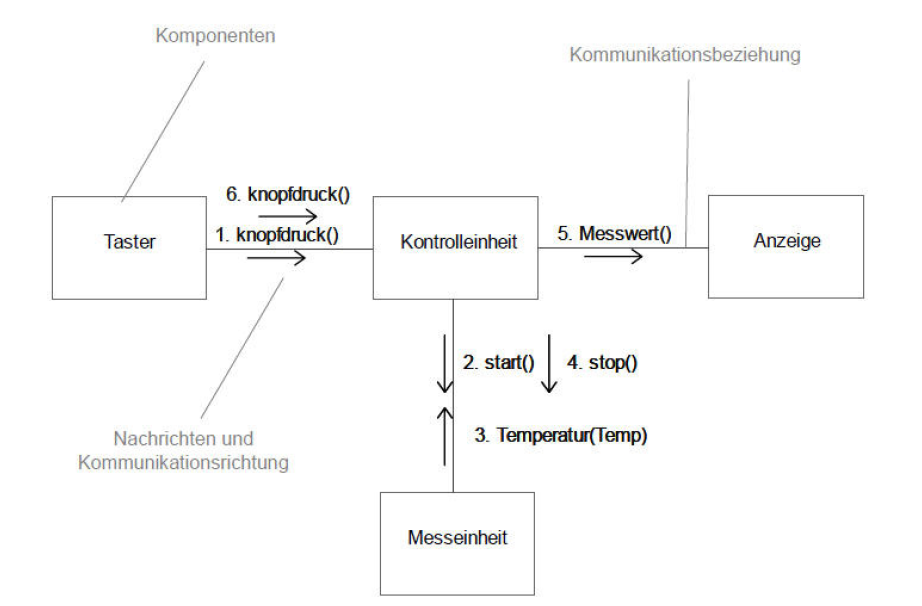
\includegraphics[height=8cm, width = 10cm,]{images/Modellierung/Kommunikationsdiagramm}
	\caption{Kommunikationsdiagramm}
\end{figure}


\subsubsection{Aktivitätsdiagramme \buch{p.42}}

\begin{multicols}{2}
	\textbf{Wird gebraucht für:}
	\begin{itemize}
		\item sequenzielle Abläufe
		\item Prozess- und Steuerfluss
		\item Auch für gleichzeitige Prozesse geeignet
		\item Weniger geeignet für komplexe logische Bedingungen (Wahrheitstabelle)
	\end{itemize}
	\columnbreak
	
	\textbf{Ideal:}
	\begin{itemize}
		\item Für kurze Zeitdauer mit einigen wenigen Objekten
		\item Bei wenigen Verschachtlungen und Verzweigungen
	\end{itemize}
\end{multicols}

\begin{minipage}[hbt]{1cm}
	\centering
	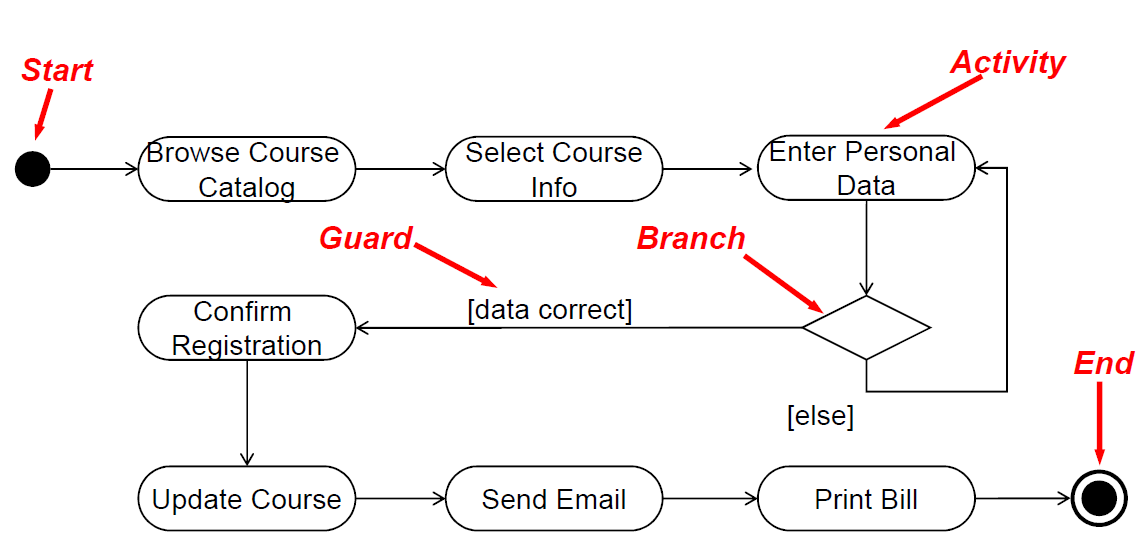
\includegraphics[height=5cm, width = 8cm,]{images/Modellierung/Aktivitaetsdiagramm1}
	\label{Bild3}
\end{minipage}
\hfill
\begin{minipage}[hbt]{8cm}
	\centering
	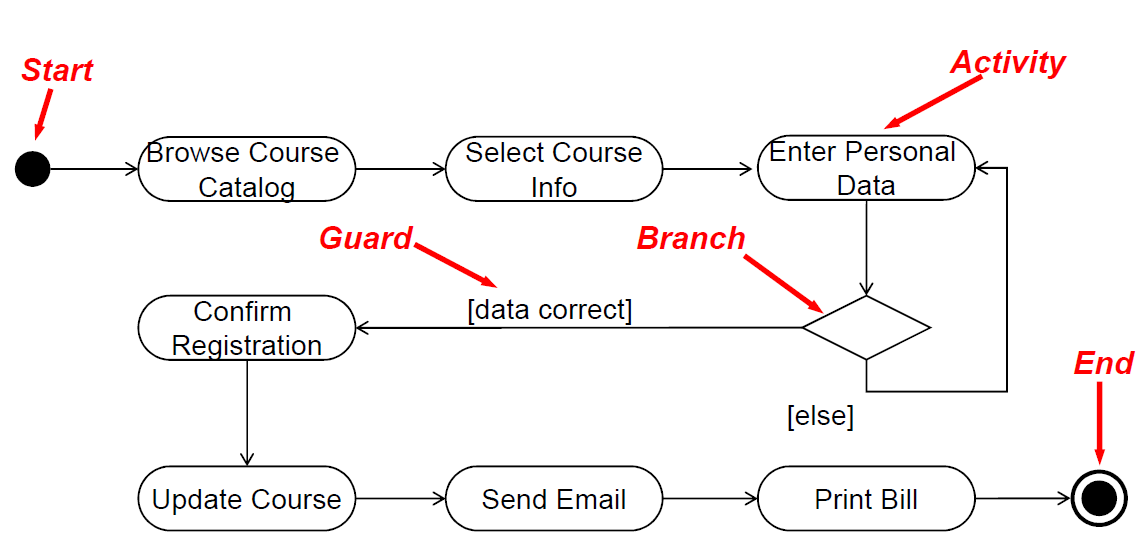
\includegraphics[height=5cm, width = 8cm,]{images/Modellierung/Aktivitaetsdiagramm1}
	\label{Bild4}
\end{minipage}



